\section{General Features of Lepton Data in \g12}\label{sec:analysis.Lepton.general}

Electron and positron energy deposition while propagating through a material was briefly explained in Sec.~\ref{sec:clas.cc} and ~\ref{sec:clas.ec}. To identify electrons and positrons properly in \abbr{CLAS}, quantities obtained from the \abbr{CC} and \abbr{EC} are used to reject charged pions. The \abbr{CC} collects the number of photo-electrons caused by Cherenkov radiation and the \abbr{EC} records the energy deposition of electrons/positrons as well as photons. A previous \abbr{CLAS} experiment \emph{g7} analyzed the properties of medium modifications from the decay of vector mesons through the leptonic decay channel. This experiment derived a set of cits for identifying electron/positrons pairs in \abbr{CLAS} by employing specific cuts to the number of photo-electrons (\abbr{NPE}) detected in the \abbr{CC}, a match in azimuthal angle $\phi$ from a charged track in the \abbr{DC} to the $\phi$ of the \abbr{CC}, as well as comparing the momentum of the charged track to the energy deposited in the \abbr{EC}. These cuts can be found in Table~\ref{tab:ISLEP_cuts}.  
\begin{table}[h!]
\begin{minipage}{\textwidth}
\begin{center}
\begin{singlespacing}

\caption[Electron/Positron PID Cuts]{\label{tab:ISLEP_cuts}Cuts applied to the \abbr{CC} and \abbr{EC} to perform electron/positron \abbr{PID} \vspace{0.75mm}}

\begin{tabular}{c|c|c}

\hline
Subsystem & Quantity & Cut \\
\hline
\multirow{2}{*}{\abbr{CC}}  & \# of photo-electrons (\abbr{NPE})  & \abbr{NPE} $>$ 2.5 \\
 &  \abbr{DC} $\phi$ \& \abbr{CC} $\phi$  & \abbr{DC} $\phi$ = \abbr{CC} $\phi$ \\
\hline
\multirow{2}{*}{\abbr{EC}}  & q$^{\pm}$ momentum threshold (p$\mathrm{_{thres}}$) & \multirow{2}{*}{p$\mathrm{_{thres}^{high}} < \ $E$\mathrm{_{calo}} <$ p$\mathrm{_{thres}^{low}}$ } \\
&  \& \abbr{EC} deposited energy (E$\mathrm{_{calo}}$) & \\
\hline \hline
\end{tabular}

%\begin{tabular}{c|c|c}
%\hline
%Subsystem & Quantity & Cut   \vspace{0.5mm} \\
%\hline
%\multirow{2}{*}{\abbr{CC}}  & \# of photo-electrons (\abbr{NPE})  & \abbr{NPE} $>$ 2.5 \\
% &  \abbr{DC} $\phi$ \& \abbr{CC} $\phi$  & \abbr{DC} $\phi$ = \abbr{CC} $\phi$ \\
%\hline
% \multirow{2}{*}{\abbr{EC}}  & q$^{\pm}$ momentum threshold (p$\mathrm{_{thres}}$) \& \abbr{EC} deposited energy (E$\mathrm{_{calo}}$)& p$\mathrm{_{thres}^{low}}$ $<$E$\mathrm{_{calo}}$ \\
%  &  q$^{\pm}$ momentum \& \abbr{EC} deposited energy  & \abbr{DC} $\phi$ = \abbr{CC} $\phi$ \\
%\hline \hline
%\end{tabular}  


\end{singlespacing}
\end{center}
\end{minipage}
\end{table}
\vspace{20pt}
To validate the \emph{g7} electron/positron \abbr{PID} scheme for \g12, a comparison of  the \abbr{CC} and \abbr{EC} quantities was performed for all charged tracks \abbr{CC}/\abbr{EC} hit signatures and while selecting events from \piz decay. To separate the \piz events from the $\pi^{+}\pi^{-}$ events, all charged pions were assigned the mass of electrons and cuts were placed on the missing energy of $\gamma p \rightarrow p e^+ e^-$ as well as a cut on the missing mass squared of $\gamma p \rightarrow p$, values found in Table~\ref{tab:lep_cuts}. A graphical depiction of the cuts applied to separate \piz events from the $\pi^{+}\pi^{-}$ events is seen in Fig.~\ref{fig:islep.cuts}.
\begin{table}[h!]
\begin{minipage}{\textwidth}
\begin{center}
\begin{singlespacing}

\caption[Cuts To Seperate \piz from $\pi^{+}\pi^{-}$ for \abbr{PID} Validation]{\label{tab:lep_cuts}Cuts applied to seperate \piz evetns from $\pi^{+}\pi^{-}$ events \vspace{0.75mm}}

\begin{tabular}{c|c|c}

\hline
Cut Topology & Topology Quantity & Value  \\
\hline
$\gamma p \rightarrow p e^+ e^-$ & Missing Energy ($\mathrm{M_E}$) & $>0.075$~GeV \\
\hline
\multirow{2}{*}{$\gamma p \rightarrow p $}  & \multirow{2}{*}{Missing mass squared ($\mathrm{M_x^2}$)} & $<$ 0.0779~GeV$^2$ for \piz events \\
&  & $>$ 0.0779~GeV$^2$ for $\pi^{+}\pi^{-}$ events\\
\hline \hline
\end{tabular}

\end{singlespacing}
\end{center}
\end{minipage}
\end{table}
\vspace{20pt} 
The values of the threshold momentum are calculated from empirical studies and are based upon calculations using the momentum obtained from the \abbr{DC }$p$ under the following criteria;
\begin{align}
\mathrm{p_{thres}^{low}} = \alpha p *(p+EC_{P\_LO})/p \nonumber \\
\mathrm{p_{thres}^{high}} = \alpha p *(p+EC_{P\_HIGH})/p \nonumber
\end{align}
where $EC_{P\_LO} = -0.3$, $EC_{P\_HIGH} = 0.5$ and  
\begin{align}
\alpha p =
\begin{cases}
.23*p + .071p^2 - .032p^3, & p<1.0 \mathrm{~GeV} \\
0.272p, & p>1.0 \mathrm{~GeV} \\
\end{cases}\nonumber
\end{align}


\begin{figure}[h!]\begin{center}
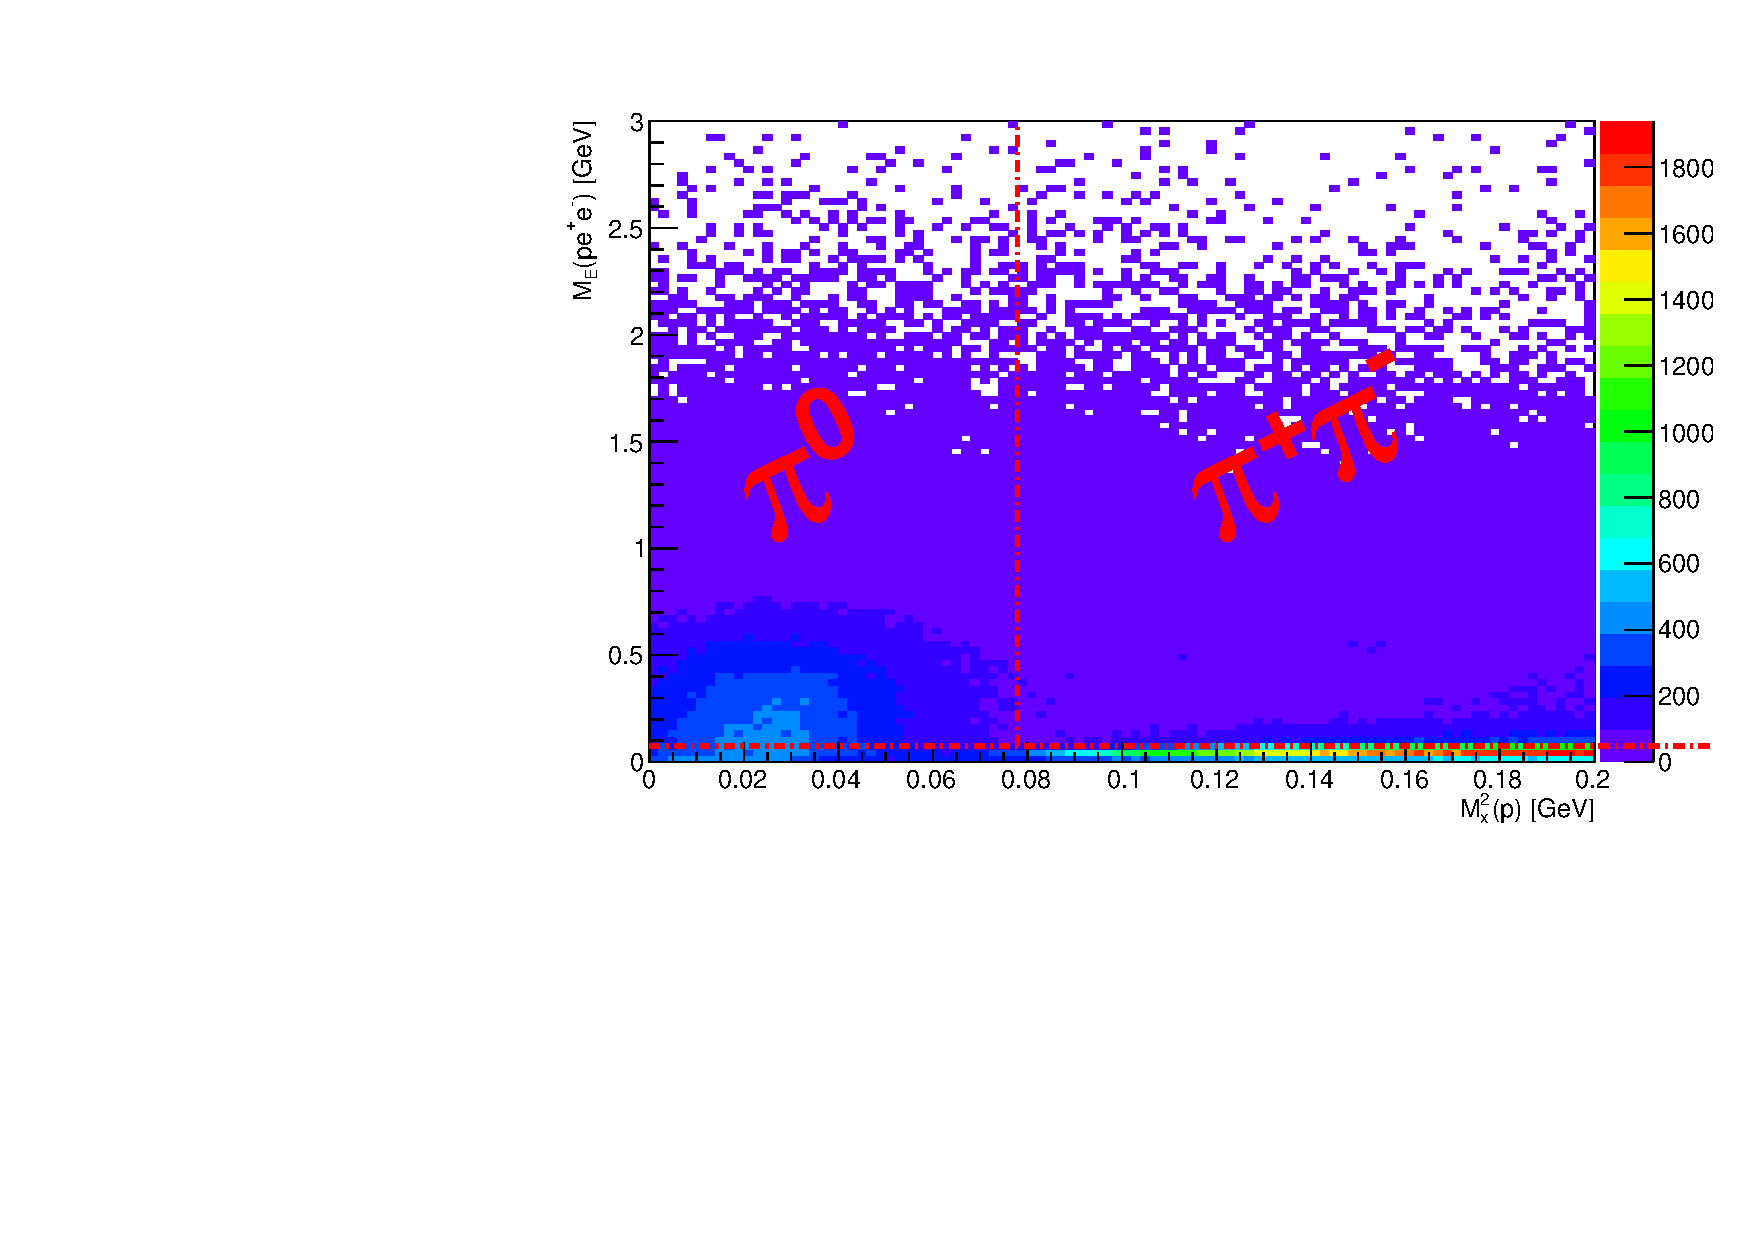
\includegraphics[width=\figwidth,height=\hfigheight]{\figures/analysis/LEP_FEATURES/Lepfeature_cuts.pdf}
\caption[Cuts Applied to Isolate \piz and $\pi^{+}\pi^{-}$ for \abbr{PID} Validation]{\label{fig:islep.cuts}Plot of missing mass squared of off proton (horizontal) vs. missing energy of proton e$^+$e$^-$ (vertical). The red dashed vertical line depicts the $\pi^{+}\pi^{-}$ threshold mass cut while the horizontal red dashed line represents the missing energy cut-off used to sepertate $\pi^{+}\pi^{-}$ from \piz.}
\end{center}\end{figure}

\subsubsection{\abbr{CC} Comparison}

The \abbr{NPE} measured by the \abbr{CC} for all positron/electron (e$^+$/e$^-$) candidates can be seen in Fig~\ref{fig:islep.CC}. The sharp decline prior to 2.5 \abbr{NPE} is due to photo-electrons created by electron/positrons, pions traveling through the \abbr{CC} or pions producing delta-electrons which pass through the \abbr{CC}. Delta-electrons are created as an effect of the ionization of gases that could be present when the pion travels through the \abbr{DC}. These types of electrons are typically lower in momentum than the electrons obtained from particle decays in \abbr{CLAS} and thus according to eq.~\ref{eq:cc.NPE} should emit less \abbr{NPE} per unit length.

Through mass conservation, as discussed in Sec.~\ref{sec:analysis.pid}, the particles in the \piz events must be e$^+$/e$^-$ pairs. In comparison to fig.~\ref{fig:islep.CC}, fig.~\ref{fig:islep.CC1} plots the \abbr{NPE} measured by the \abbr{CC} for all e$^+$/e$^-$ pairs for \piz events selected as shown in fig.~\ref{fig:islep.cuts}. It can be seen that the sharp decline prior to \abbr{NPE} = 2.5 is reduced leaving mostly electrons or positrons signatures in the \abbr{CC} concluding that the \emph{g7} \abbr{CC} \abbr{NPE} cut is valid for identifying e$^+$/e$^-$ pairs while rejecting $\pi^+$/$\pi^-$ pairs.
 
%
\begin{figure}[h!]\begin{center}
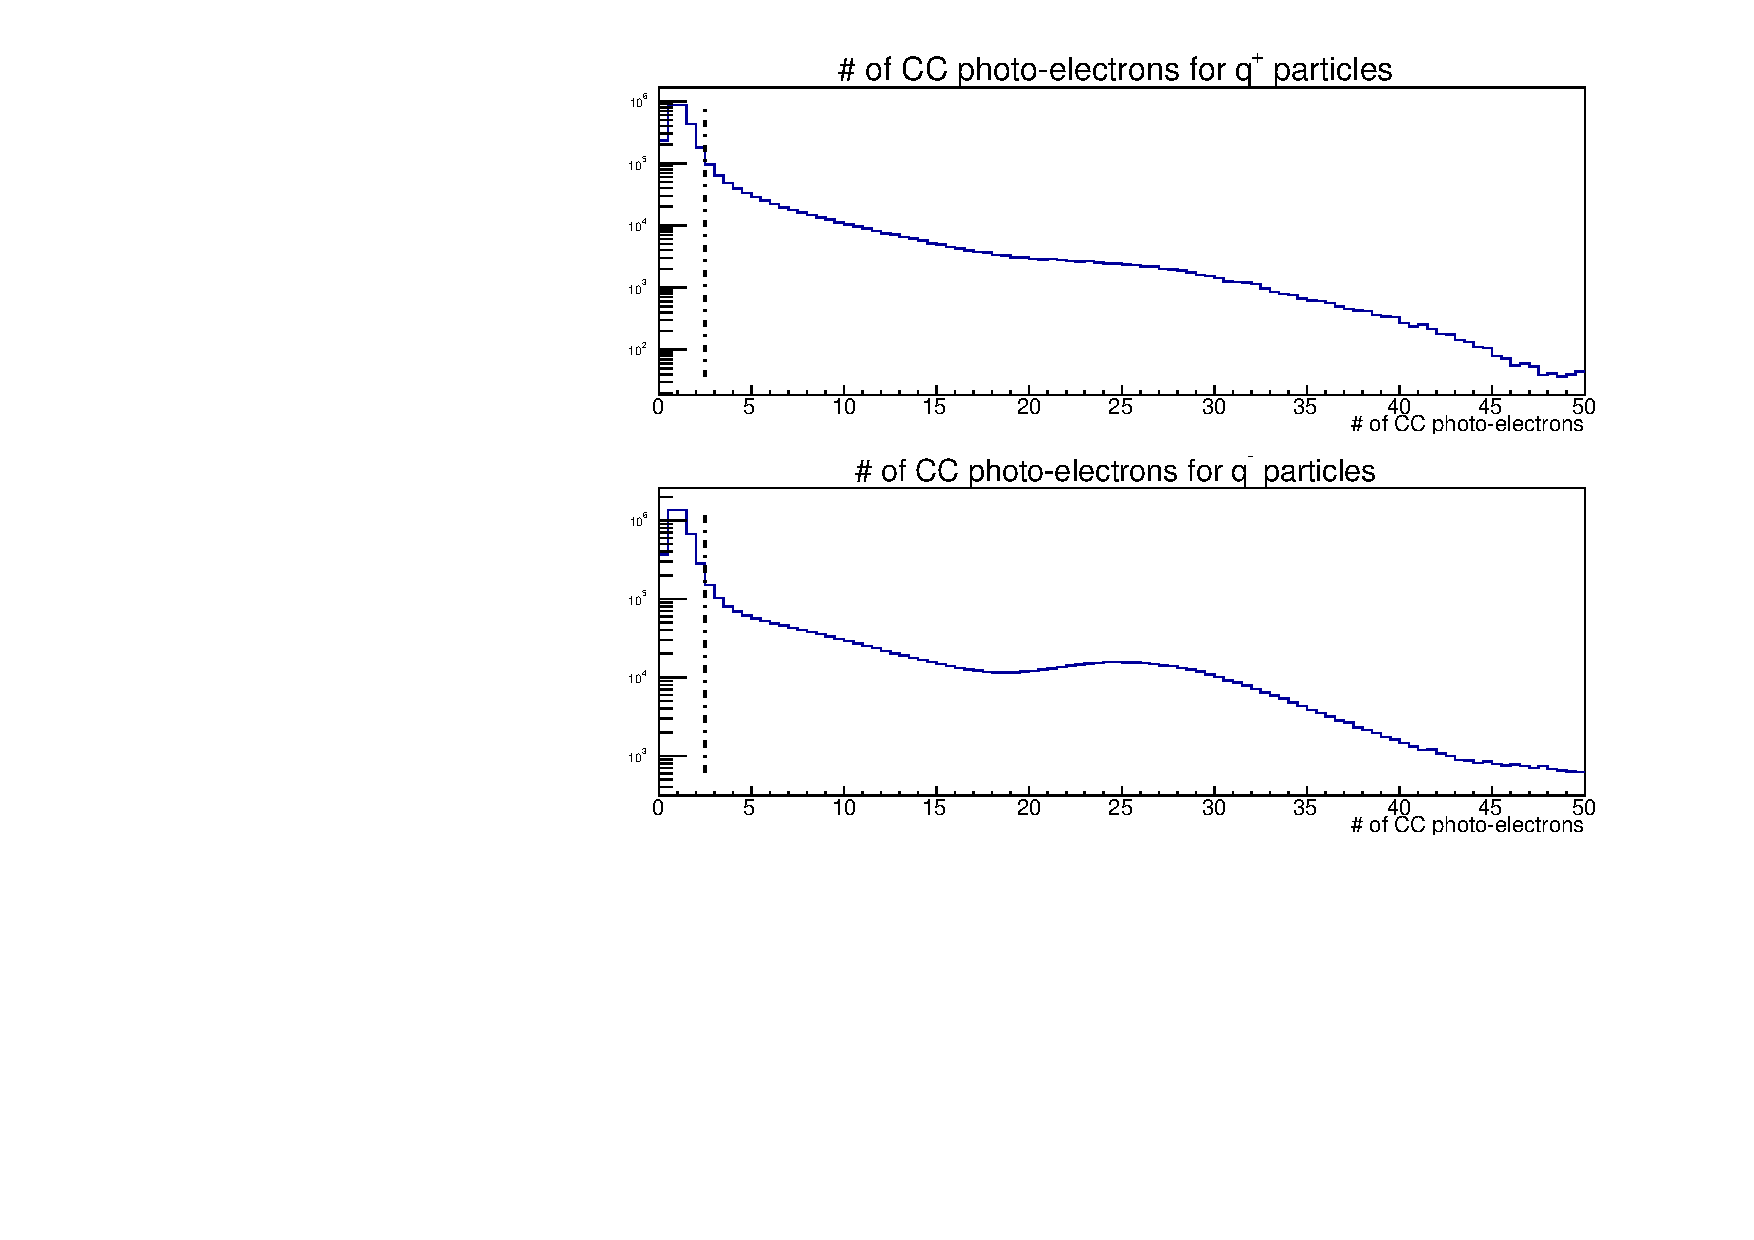
\includegraphics[width=\figwidth,height=\hfigheight]{\figures/analysis/LEP_FEATURES/CC_nPE.pdf}
\caption[Number of Photo-electrons Measured by \abbr{CC} for All e$^-$ and e$^+$ Candidates]{\label{fig:islep.CC}Plot of \abbr{NPE} measured by \abbr{CLAS} \abbr{CC} subsystem for positron/electron candidates top/bottom respectively. The dashed dotted vertical line depicts the cut applied if using the \emph{g7} lepton \abbr{PID} scheme.}
\end{center}\end{figure}

\begin{figure}[h!]\begin{center}
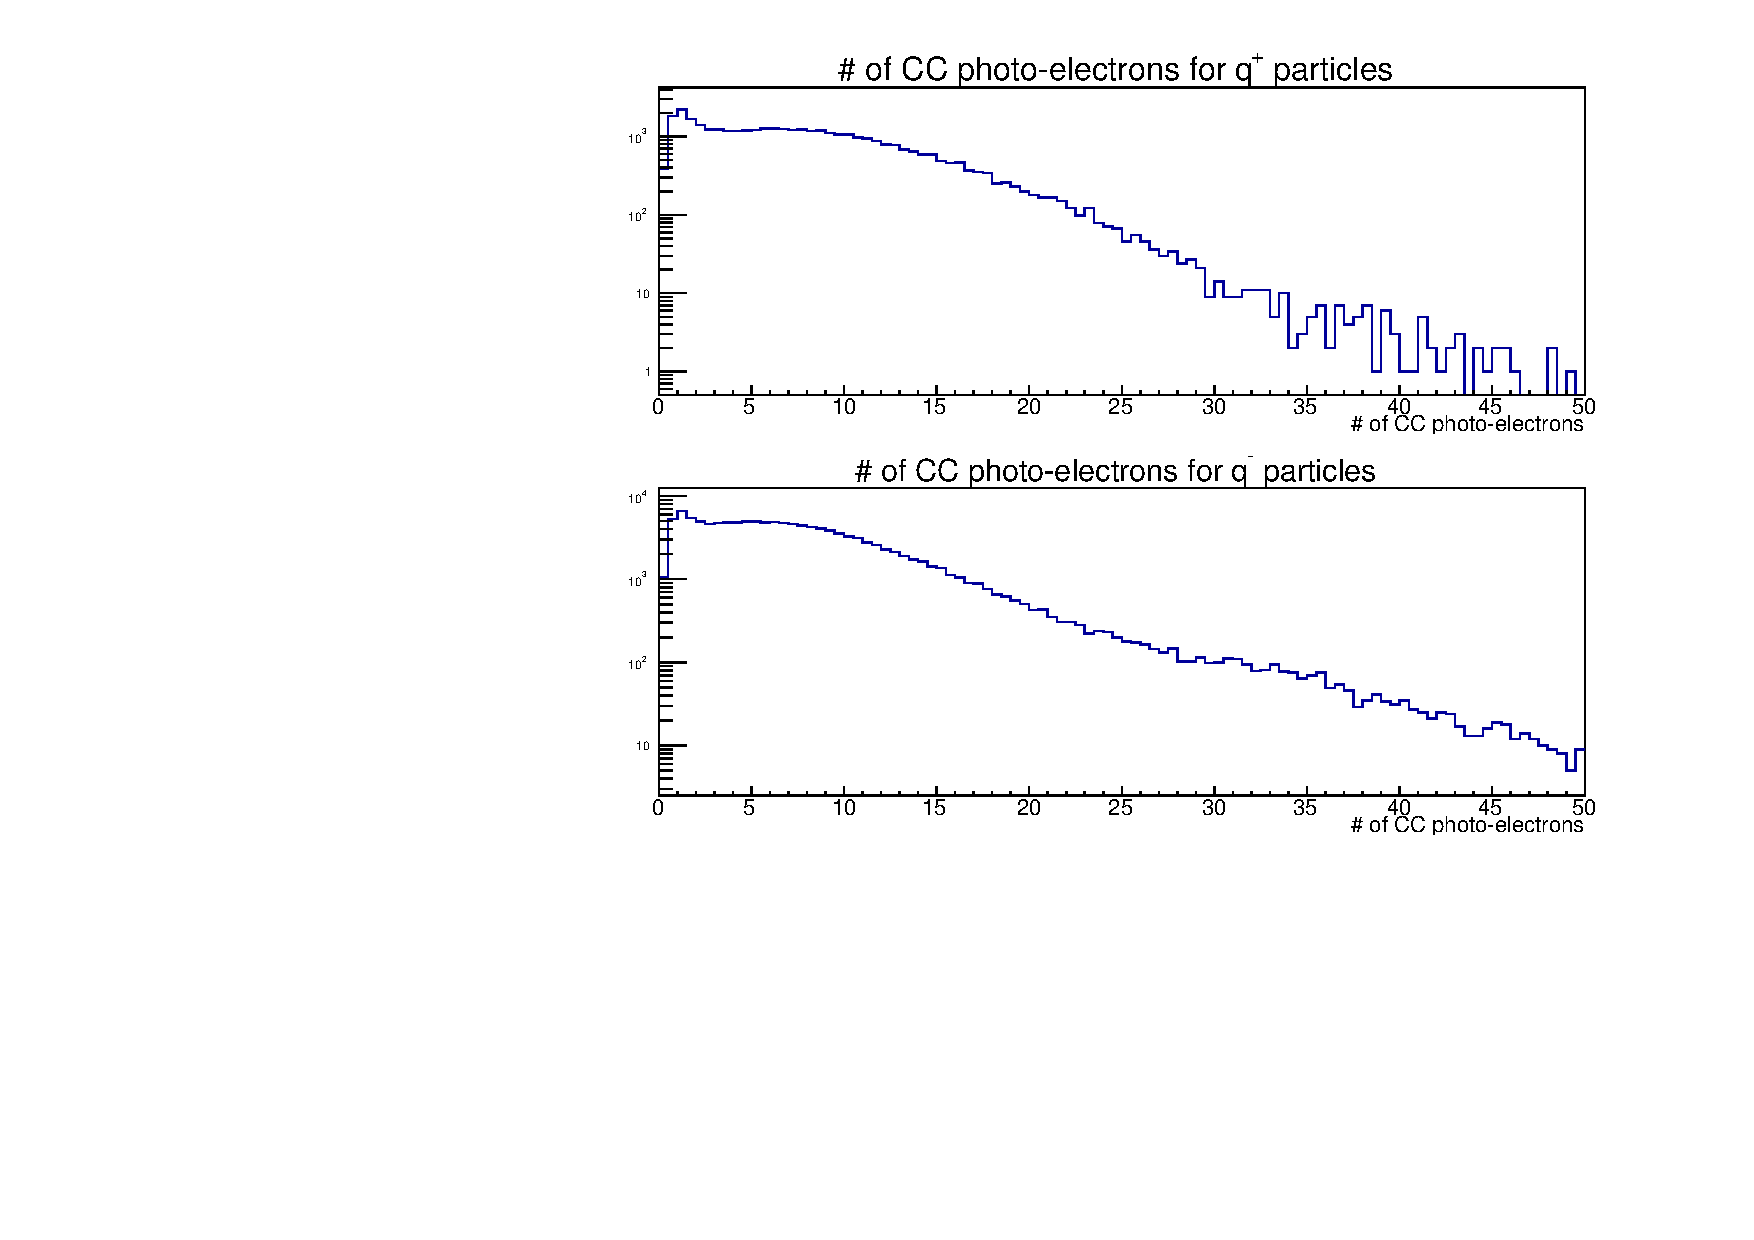
\includegraphics[width=\figwidth,height=\hfigheight]{\figures/analysis/LEP_FEATURES/CC_NPEcut.pdf}
\caption[Number of Photo-electrons Measured by \abbr{CC} for \piz Events]{\label{fig:islep.CC1}Plot of \abbr{NPE} measured by \abbr{CLAS} \abbr{CC} subsystem when selecting \piz events seen in Fig~\ref{fig:islep.cuts}, positron/electron candidates top/bottom respectively.}
\end{center}\end{figure}
\FloatBarrier
\subsubsection{\abbr{EC} Comparison}
%EC
%
%e-
%

Similarly to the \abbr{CC} comparison, figures~\ref{fig:islep.pimEClow},~\ref{fig:islep.pimEChigh},~\ref{fig:islep.pipEClow},~\ref{fig:islep.pipEChigh} depict the  p$\mathrm{_{thres}^{low}}$ and  p$\mathrm{_{thres}^{low}}$ cuts listed in  Table~\ref{tab:ISLEP_cuts} for the q$^-$ and q$^+$ tracks respectively. After \piz event selection, seen in figures~\ref{fig:islep.pimEC},~\ref{fig:islep.pimECcut} ,~\ref{fig:islep.pipEC} ,~\ref{fig:islep.pipECcut}, the bulk of e$^+$/e$^-$ events reside within the region of the cut acceptance therefore it is evident that the \emph{g7} \abbr{EC} cuts are valid for identifying e$^+$/e$^-$ pairs. The following four plots are for electron($e^-$) \abbr{PID} validation of the \emph{g7} \abbr{EC} cuts described in Table~\ref{tab:ISLEP_cuts}.
%
\begin{figure}[h!]\begin{center}
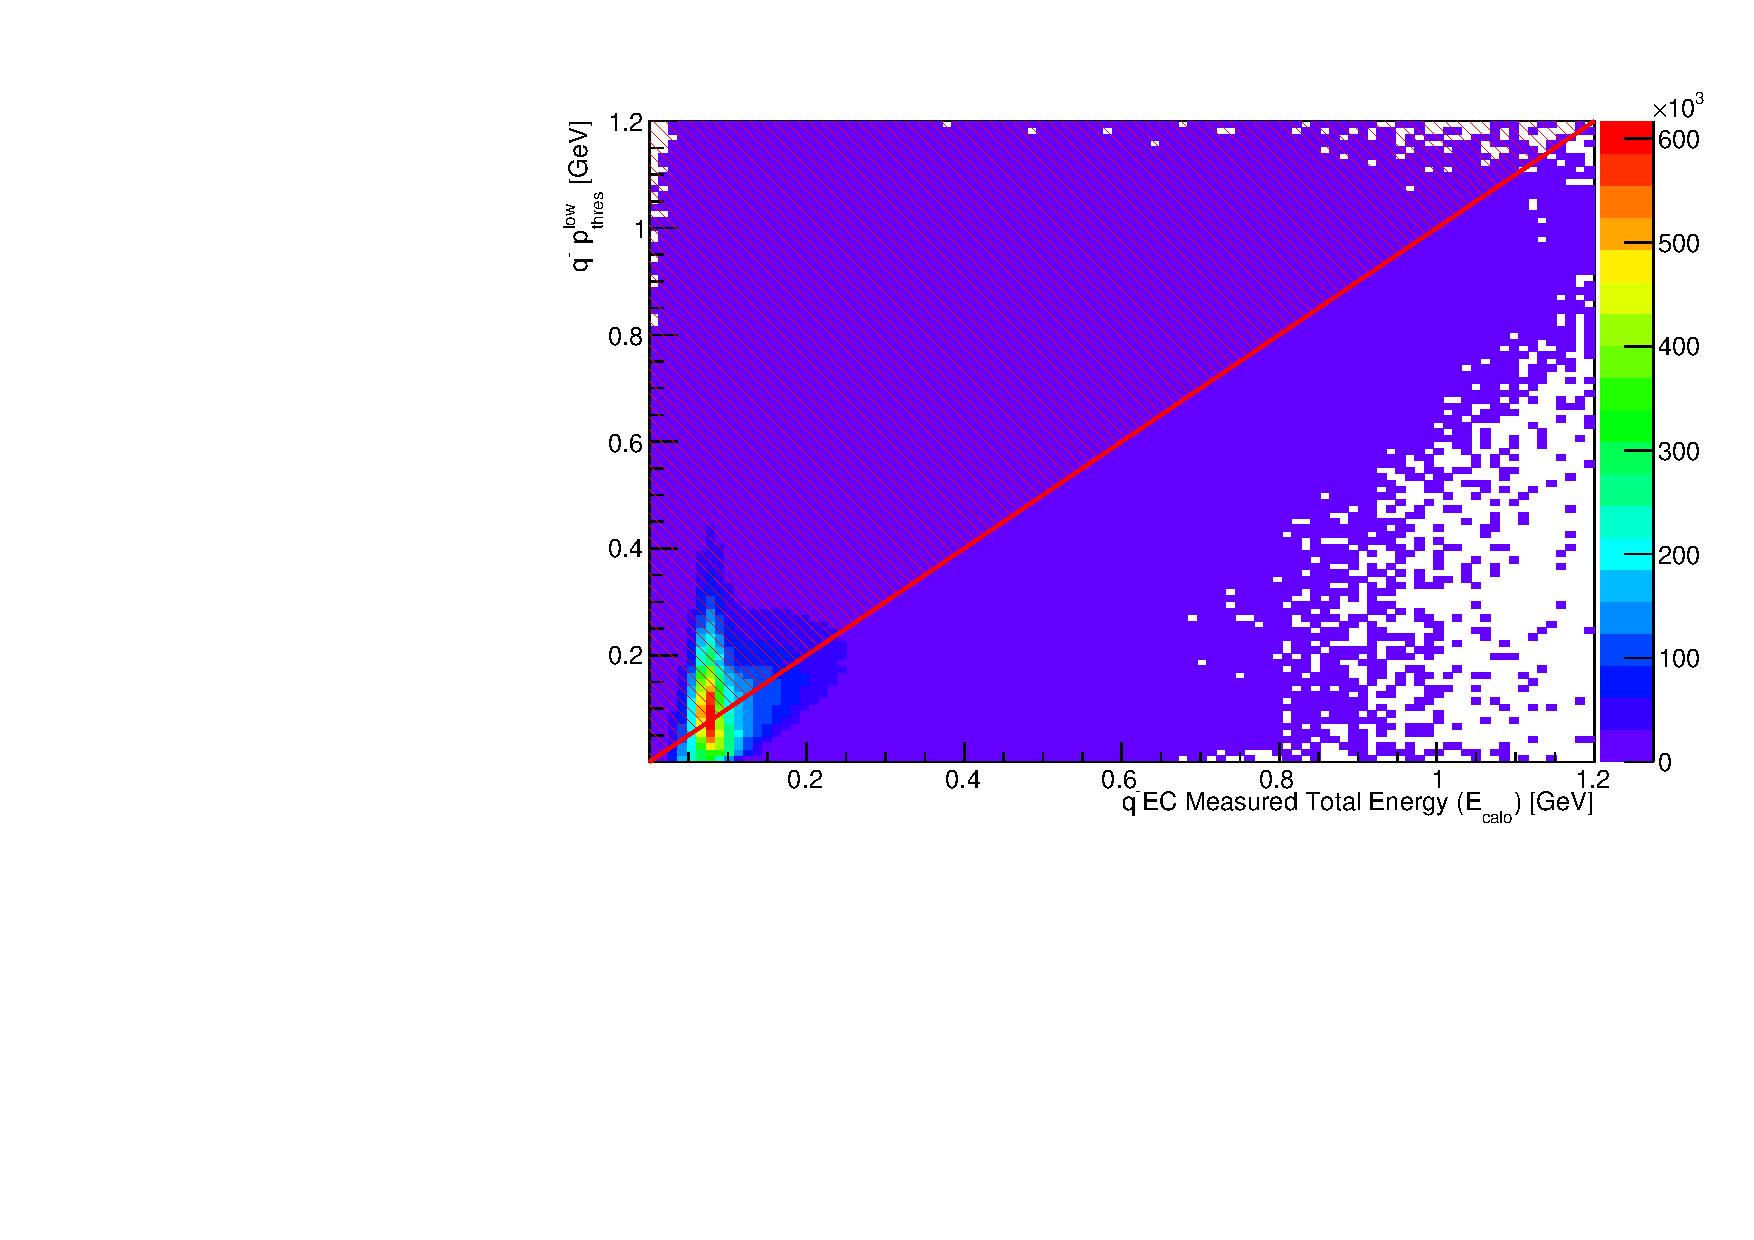
\includegraphics[width=\figwidth,height=0.7\hfigheight]{\figures/analysis/LEP_FEATURES/Pim_EClow.pdf}
\caption[\abbr{EC} Deposited Energy Comparison to Lower Threshold Track Momentum for q$^-$ Tracks]{\label{fig:islep.pimEClow}Plot of energy deposited measured by \abbr{EC} vs. track momentum p$\mathrm{_{thres}^{low}}$ for negative charged tracks. The red region depicts the cut that would reject events in the \emph{g7} lepton \abbr{EC} \abbr{PID} scheme.}
\end{center}\end{figure}

\begin{figure}[h!]\begin{center}
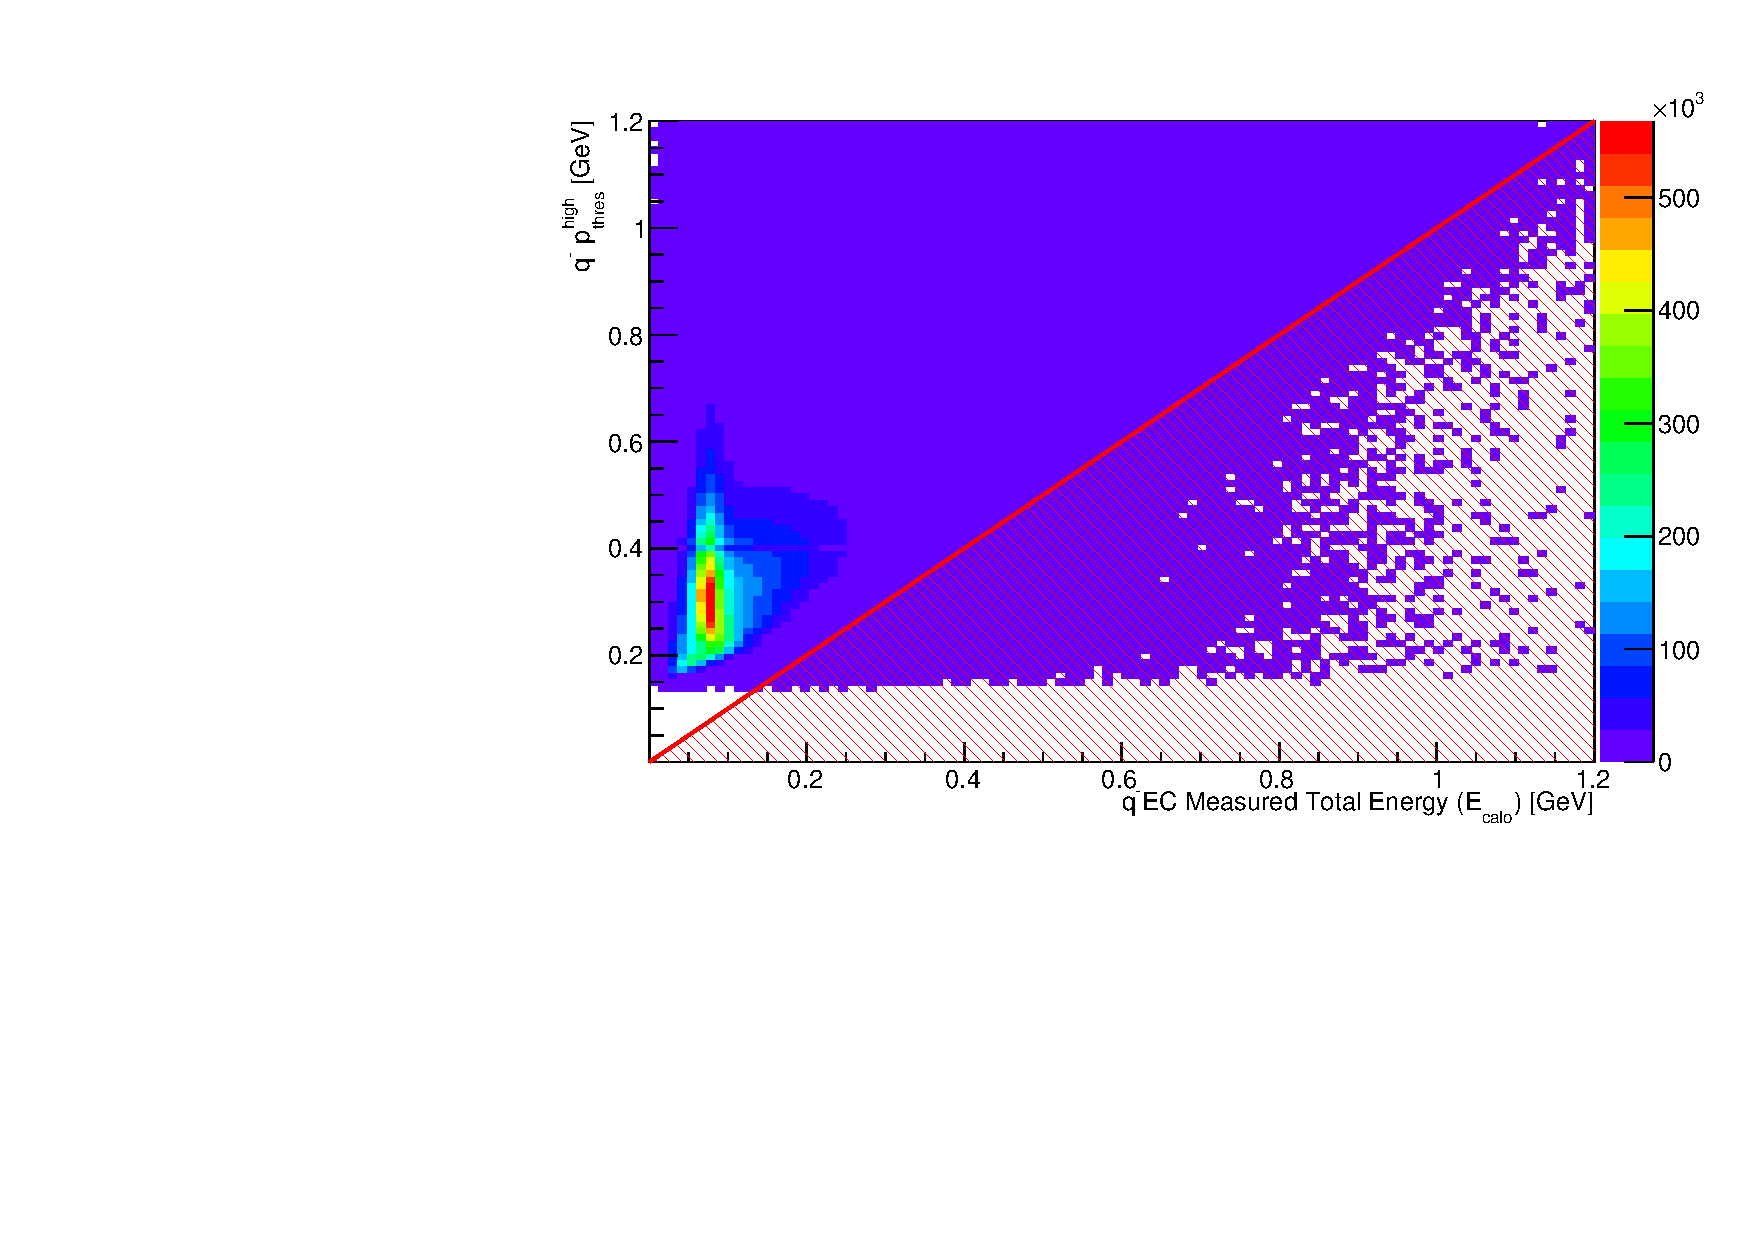
\includegraphics[width=\figwidth,height=0.7\hfigheight]{\figures/analysis/LEP_FEATURES/Pim_EChigh.pdf}
\caption[\abbr{EC} Deposited Energy Comparison to Upper Threshold Track Momentum for q$^-$ Tracks]{\label{fig:islep.pimEChigh}Plot of energy deposited measured by \abbr{EC} vs. track momentum p$\mathrm{_{thres}^{high}}$ for negative charged tracks. The red region depicts the cut that would reject events in the \emph{g7} lepton \abbr{EC} \abbr{PID} scheme.}
\end{center}\end{figure}


\begin{figure}[h!]\begin{center}
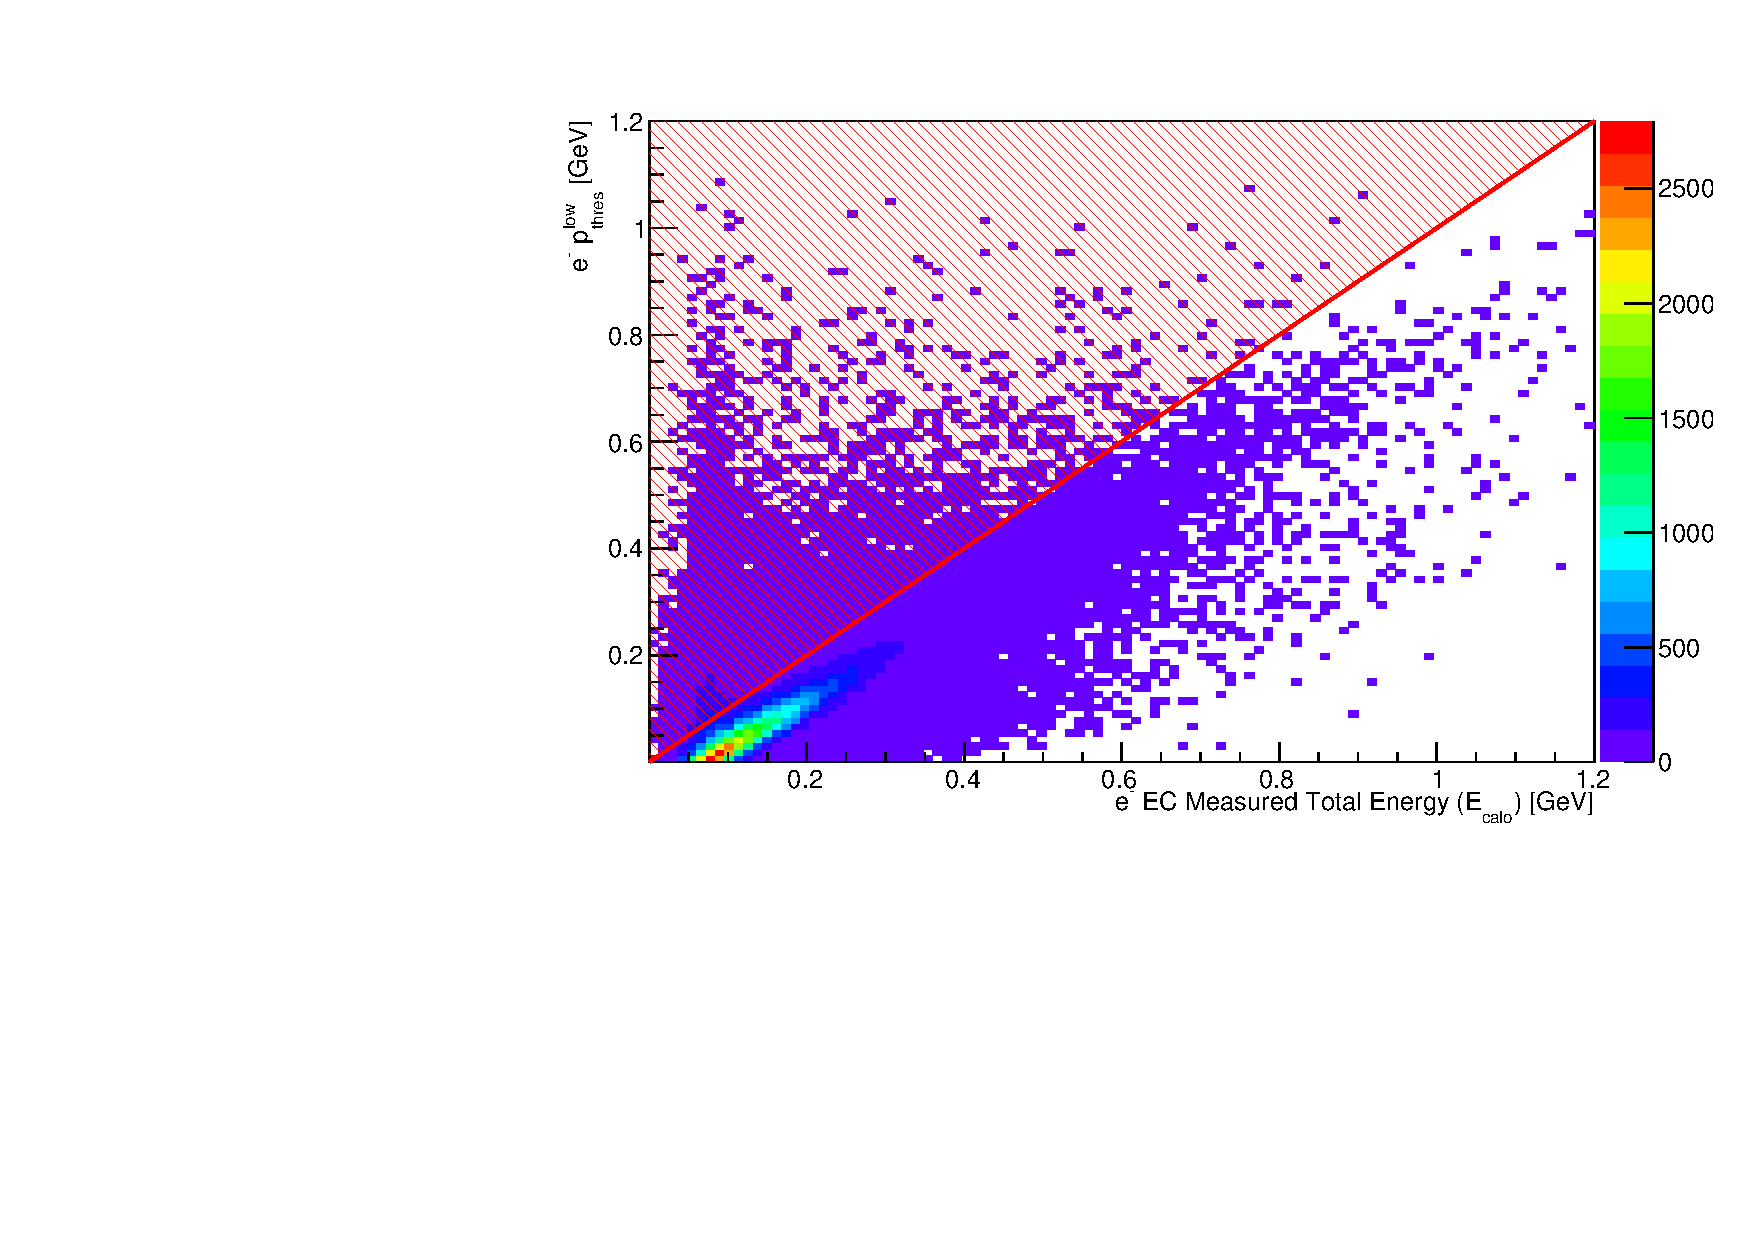
\includegraphics[width=\figwidth,height=0.7\hfigheight]{\figures/analysis/LEP_FEATURES/Pim_EClowcut.pdf}
\caption[\abbr{EC} Deposited Energy Comparison to Track Momentum for e$^-$ Candidates]{\label{fig:islep.pimEC}Plot of energy deposited measured by \abbr{EC} vs. track momentum p$\mathrm{_{thres}^{low}}$ for electrons from \piz events without the \emph{g7} lepton \abbr{EC} \abbr{PID} scheme applied. The red region depicts the cut that would reject events in the \emph{g7} lepton \abbr{EC} \abbr{PID} scheme.}
\end{center}\end{figure}

\begin{figure}[h!]\begin{center}
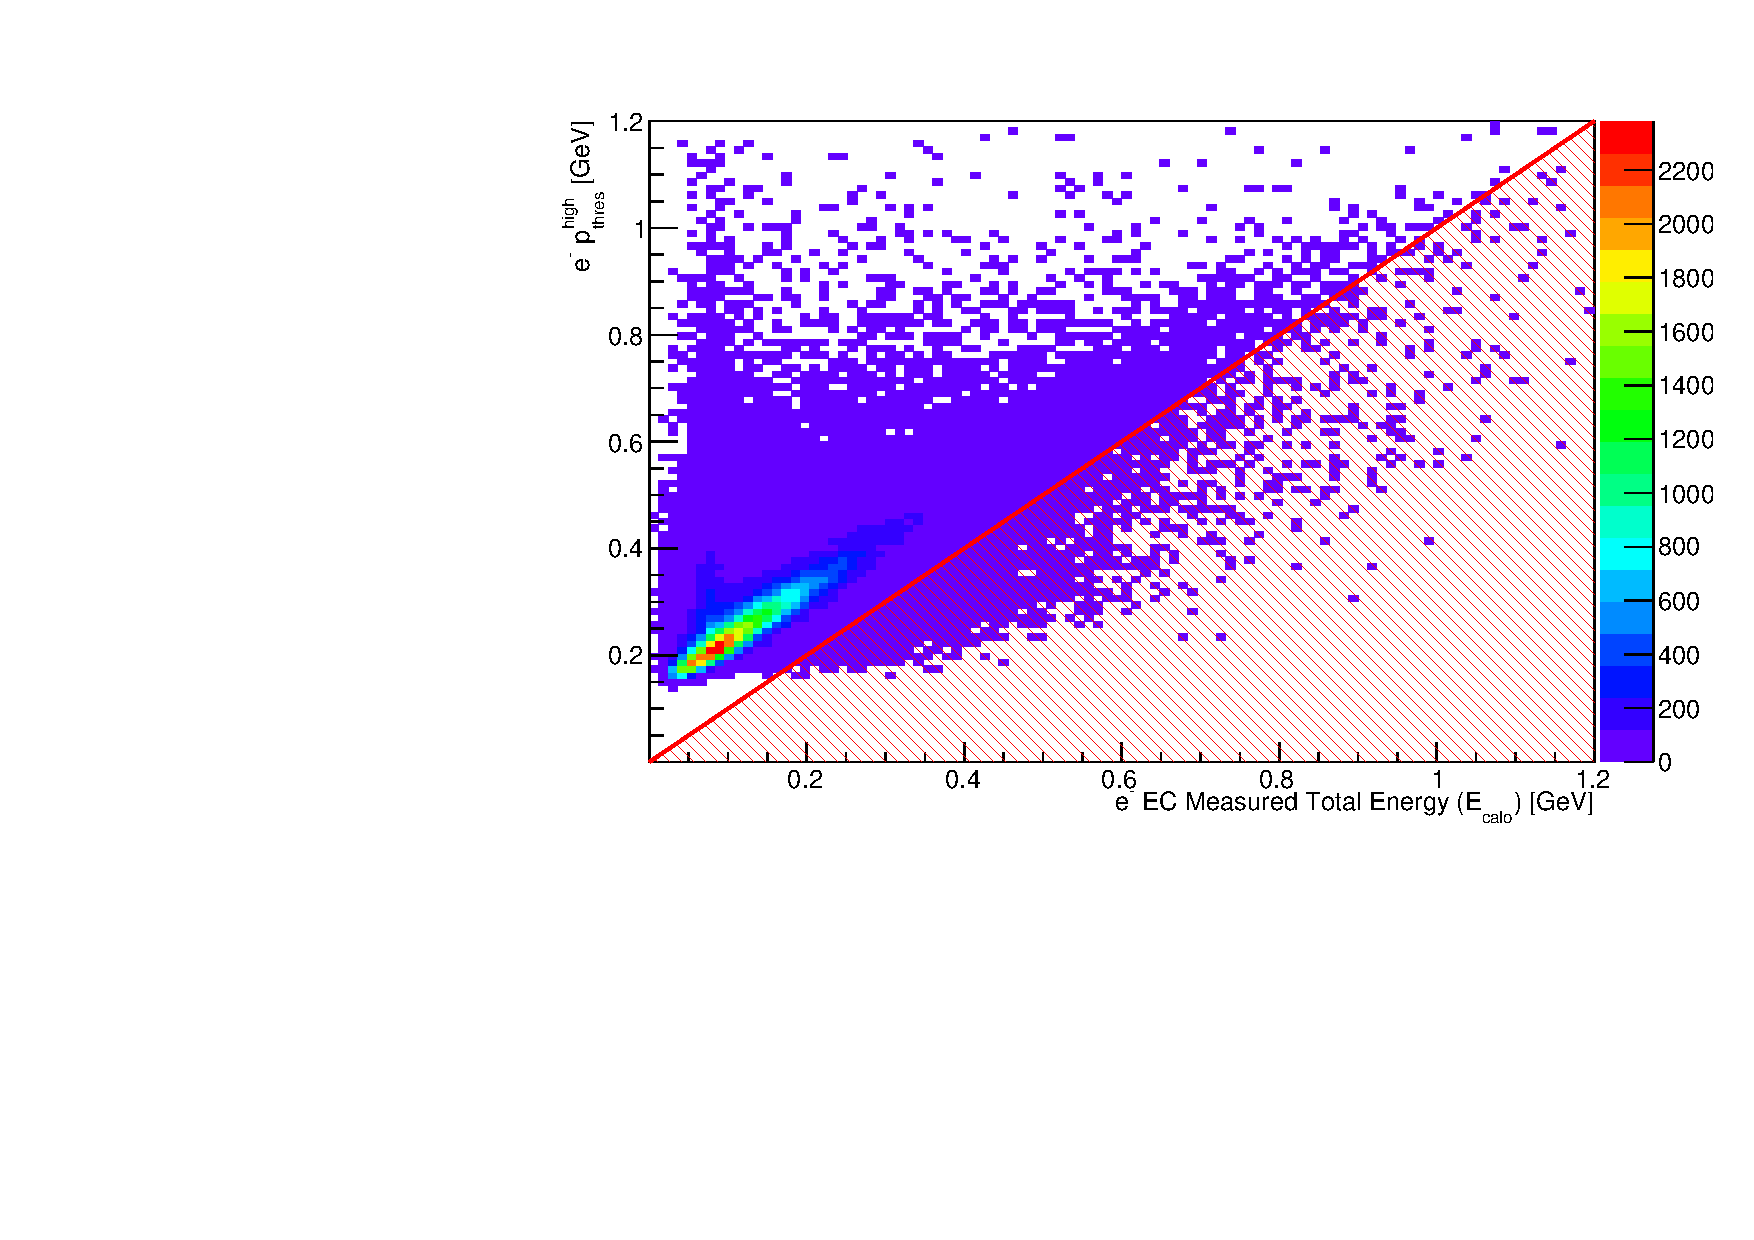
\includegraphics[width=\figwidth,height=0.7\hfigheight]{\figures/analysis/LEP_FEATURES/Pim_EChighcut.pdf}
\caption[\abbr{EC} Deposited Energy Comparison to Track Momentum for e$^-$ from \piz Events]{\label{fig:islep.pimECcut}Plot of energy deposited measured by \abbr{EC} vs. track momentum p$\mathrm{_{thres}^{high}}$ for electrons from \piz events without the \emph{g7} lepton \abbr{EC} \abbr{PID} scheme applied. The red region depicts the cut that would reject events in the \emph{g7} lepton \abbr{EC} \abbr{PID} scheme.}
\end{center}\end{figure}
\FloatBarrier
The following four plots are for positron($e^+$) \abbr{PID} validation of the \emph{g7} \abbr{EC}
cuts described in Table~\ref{tab:ISLEP_cuts}.
%
%
%e+
%
%
\begin{figure}[h!]\begin{center}
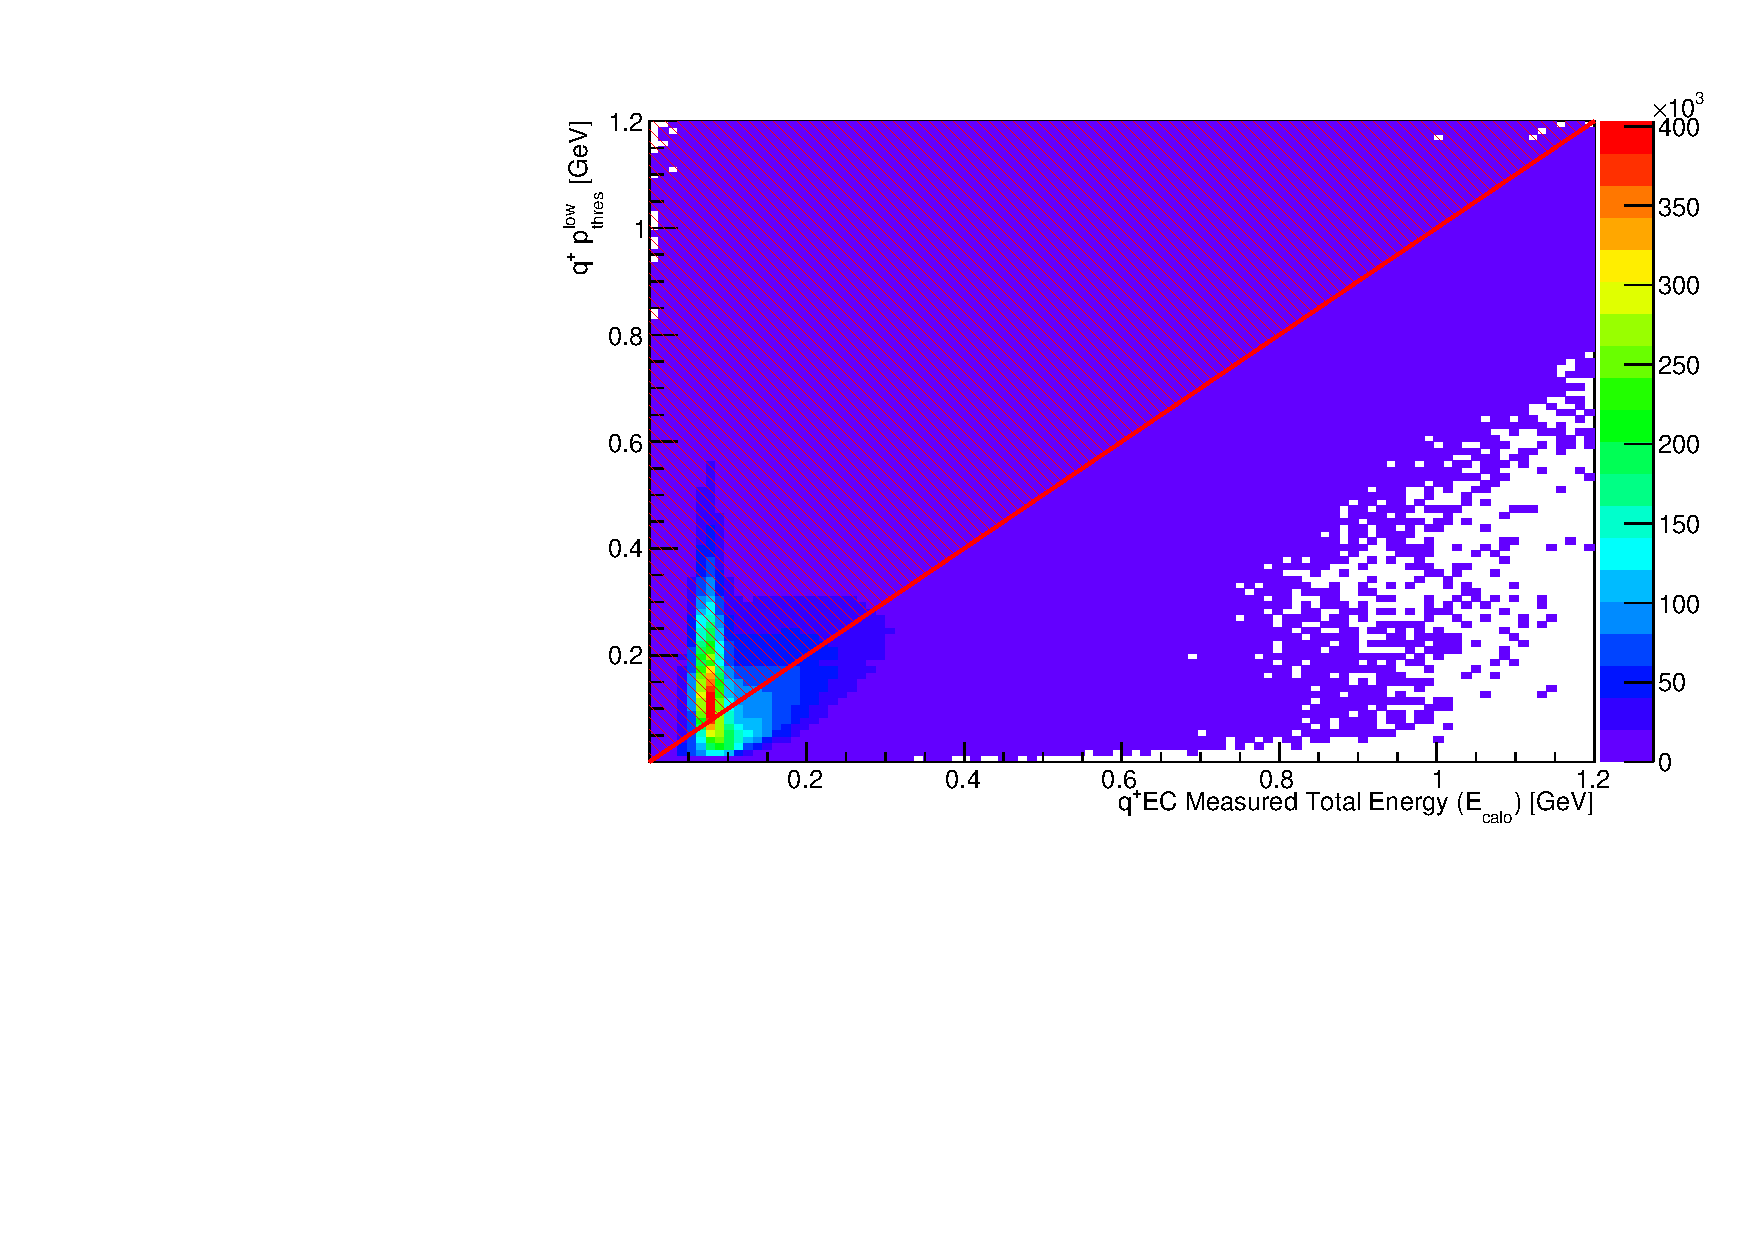
\includegraphics[width=\figwidth,height=0.7\hfigheight]{\figures/analysis/LEP_FEATURES/Pip_EClow.pdf}
\caption[\abbr{EC} Deposited Energy Comparison to Lower Threshold Track Momentum for q$^+$ Tracks]{\label{fig:islep.pipEClow}Plot of energy deposited measured by \abbr{EC} vs. track momentum p$\mathrm{_{thres}^{low}}$ for positive charged tracks. The red region depicts the cut that would reject events in the \emph{g7} lepton \abbr{EC} \abbr{PID} scheme.}
\end{center}\end{figure}

\begin{figure}[h!]\begin{center}
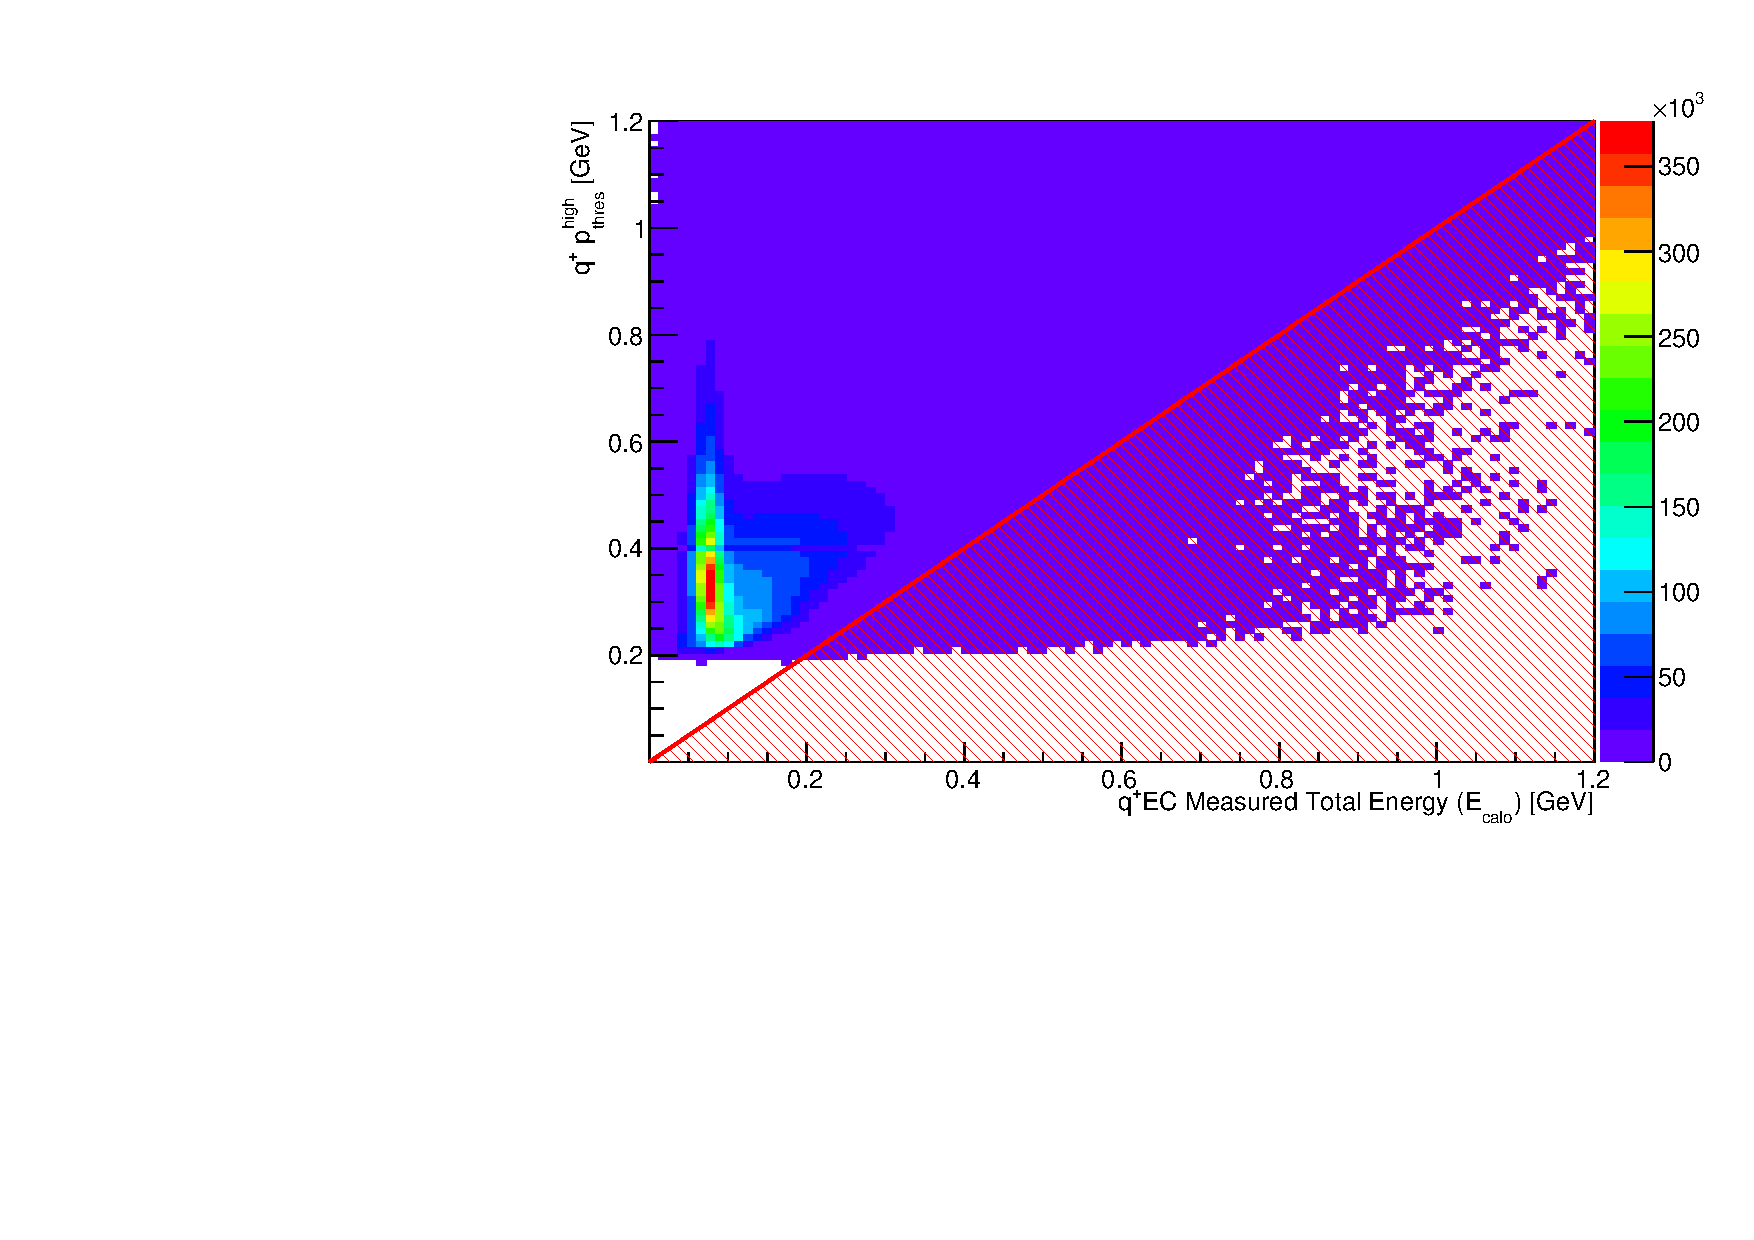
\includegraphics[width=\figwidth,height=0.7\hfigheight]{\figures/analysis/LEP_FEATURES/Pip_EChigh.pdf}
\caption[\abbr{EC} Deposited Energy Comparison to Upper Threshold Track Momentum for q$^+$ Tracks]{\label{fig:islep.pipEChigh}Plot of energy deposited measured by \abbr{EC} vs. track momentum p$\mathrm{_{thres}^{high}}$ for positive charged tracks. The red region depicts the cut that would reject events in the \emph{g7} lepton \abbr{EC} \abbr{PID} scheme.}
\end{center}\end{figure}

\begin{figure}[h!]\begin{center}
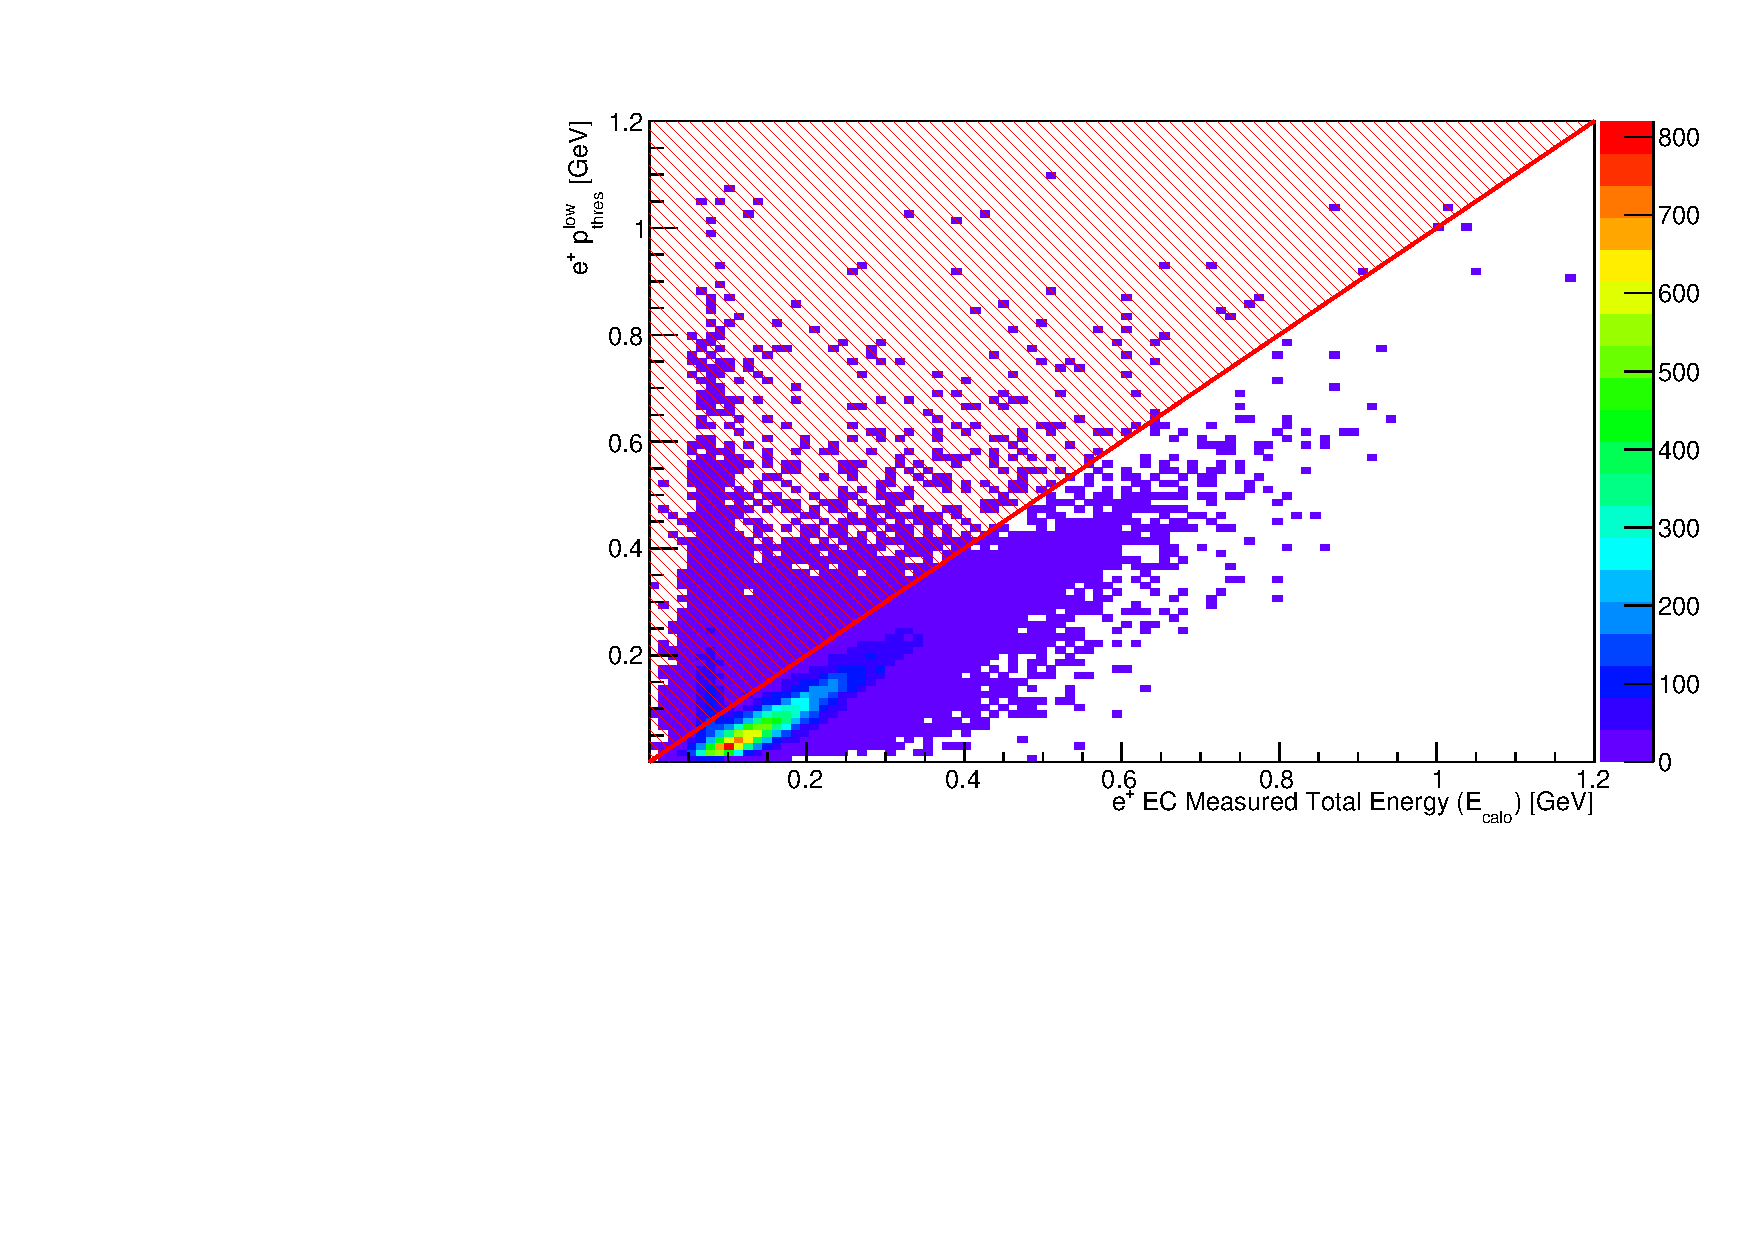
\includegraphics[width=\figwidth,height=0.7\hfigheight]{\figures/analysis/LEP_FEATURES/Pip_EClowcut.pdf}
\caption[\abbr{EC} Deposited Energy Comparison to Track Momentum for e$^+$ Candidates]{\label{fig:islep.pipEC}Plot of energy deposited measured by \abbr{EC} vs. track momentum p$\mathrm{_{thres}^{low}}$ for positrons from \piz events without the \emph{g7} lepton \abbr{EC} \abbr{PID} scheme applied. The red region depicts the cut that would reject events in the \emph{g7} lepton \abbr{EC} \abbr{PID} scheme.}
\end{center}\end{figure}

\begin{figure}[h!]\begin{center}
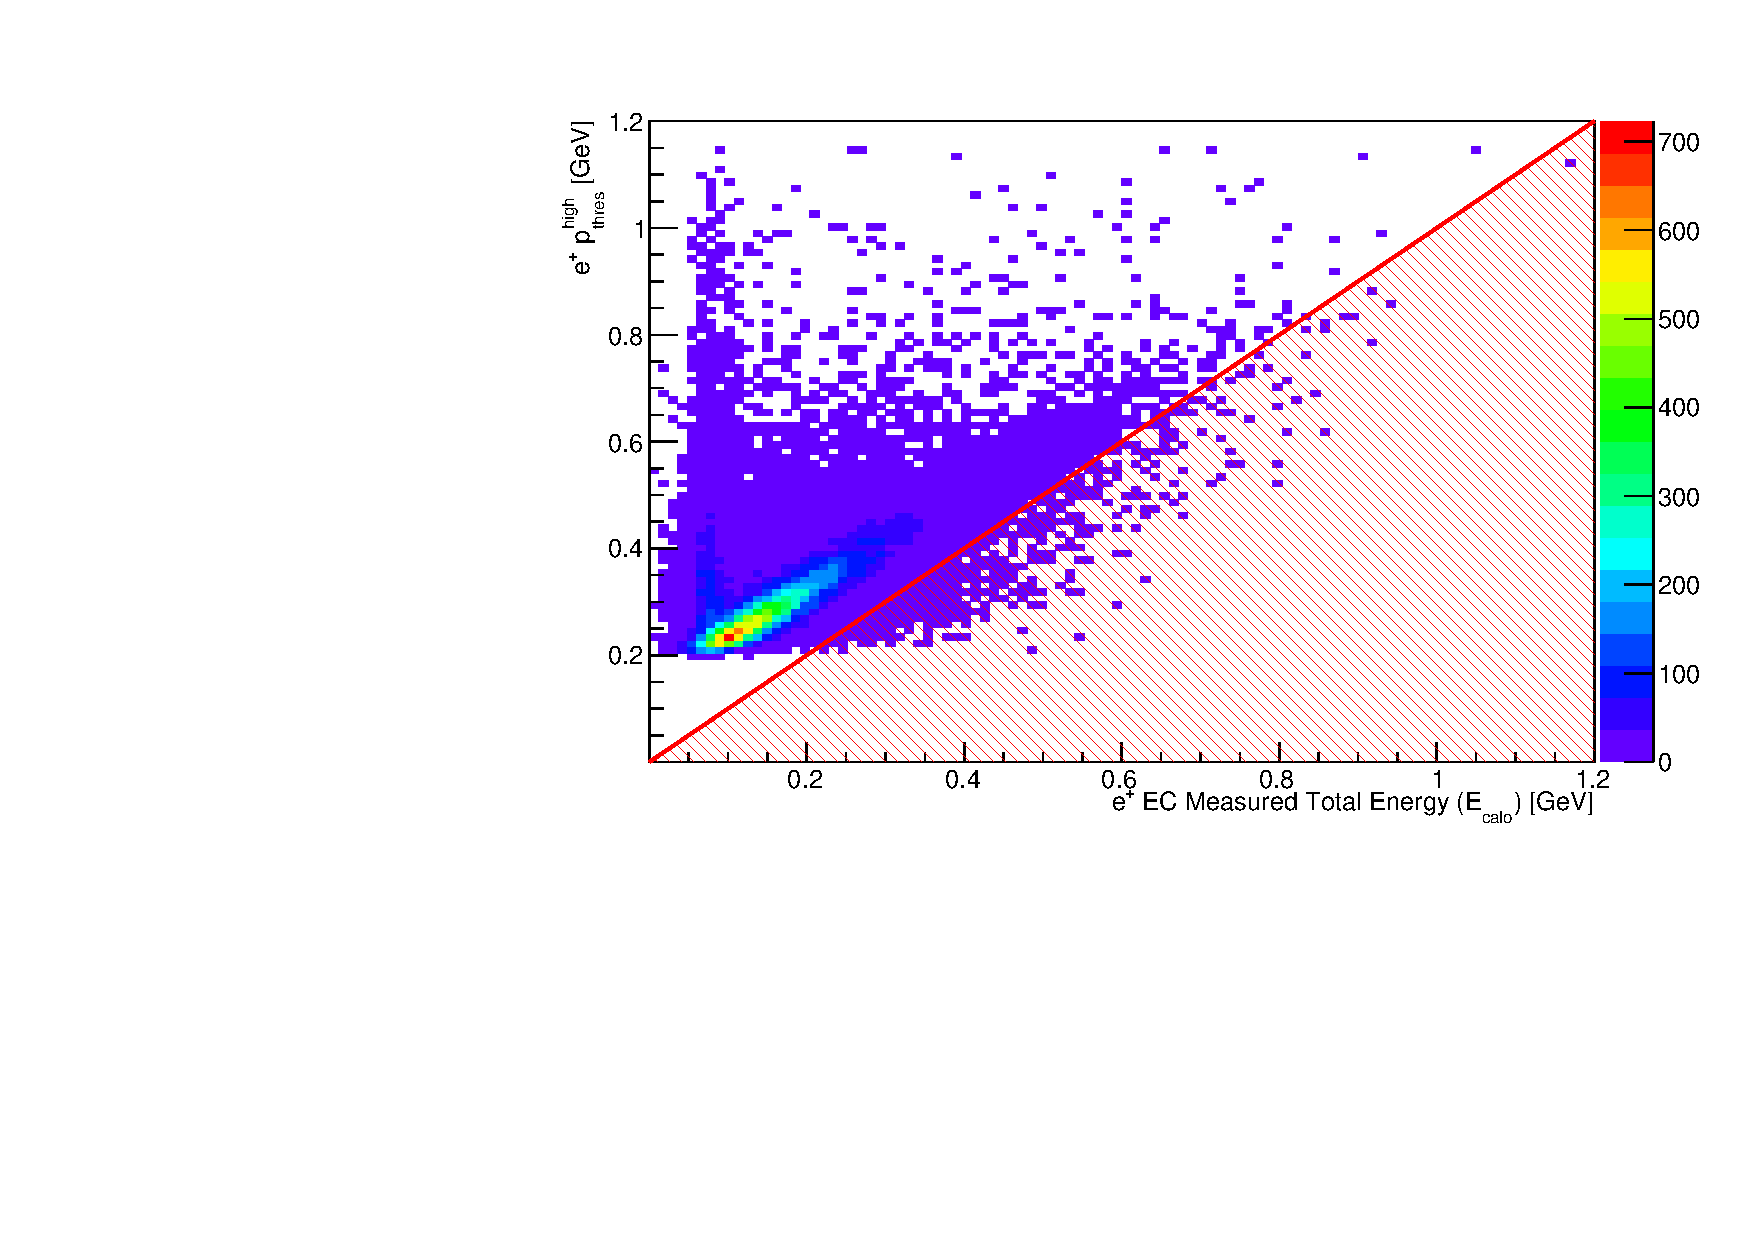
\includegraphics[width=\figwidth,height=0.7\hfigheight]{\figures/analysis/LEP_FEATURES/Pip_EChighcut.pdf}
\caption[\abbr{EC} Deposited Energy Comparison to Track Momentum for e$^+$ from \piz Events]{\label{fig:islep.pipECcut}Plot of energy deposited measured by \abbr{EC} vs. track momentum p$\mathrm{_{thres}^{high}}$ for positrons from \piz events without the \emph{g7} lepton \abbr{EC} \abbr{PID} scheme applied. The red region depicts the cut that would reject events in the \emph{g7} lepton \abbr{EC} \abbr{PID} scheme.}
\end{center}\end{figure}
%


\FloatBarrier
